\chapter{Einleitung}
Seit einigen Jahren findet man immer häufiger Bedienungen mit Touchscreens.
Ihr Einsatzbereich scheint keine Grenzen zu haben und so hat sich die Technologie in den letzten Jahren rasant weiterentwickelt.


\section{Ziel des Projekts}
In dieser Projektarbeit ist es Ziel, die Aufnahme und Auswertung der Koordinaten mittels eines resistiven Touchscreen.
Zum Schluss soll die Steuerung noch dahingehend erweitert werden, dass damit die Maus eines PC's gesteuert wird.


\section{Grundlagen}
\subsection{Resistives Touchscreen}
Es gibt bei den resistiven Touchscreens zwei unterschiedliche Gruppen.
Zum einen gibt es 4-Wire resistive Touchscreens.
Diese haben vier Anschlüsse, über die die Positionsauswertung läuft.
Zudem gibt es noch die 5-Wire resistive Touchscreens.
Hier sind fünf Anschlüsse, über die die Positionsauswertung durchgeführt wird.

Bei einem 4-Wire resistiven Touchscreen gibt es zwei Ebenen, bei denen die obere auf die untere gedrückt werden kann.
Eine Ebene ist mit Elektronen geladen und über die andere Ebene misst man die Spannung die in eine Richtung bei der Berührung abfällt.
Für die andere Richtung ist es gespiegelt.
Die Ebene, die die Spannung in eine Richtung misst, ist für die andere Richtung mit Elektronen geladen.
Die Messung wird dann von der anderen Ebene durchgeführt.
Über die unterschiedlichen Beträge der Spannung lässt sich dann die Koordinate in x-Richtung und y-Richtung bestimmen.

Die 5-Wire resistive Touchscreens haben ebenfalls zwei Ebene.
Der Unterschied zu den 4-Wire Touchscreen liegt darin, dass es nur eine Ebene gibt, die geladen ist.
Normalerweise ist es die untere Schicht.
Die obere Schicht misst  für x-Richtung und y-Richtung die abfallende Spannung.
Auch hier wird durch Druck auf die obere Schicht ein Kontakt zwischen den beiden Ebenen erstellt, damit die Messung durchgeführt werden kann.

Die 5-Wire Touchscreens sind gegenüber den 4-Wire Widerstandsfähiger und haben dadurch eine längere Lebenserwartung.\cite{5w4w}

In diesem Projekt wird ein 4-Wire resistiver Touchscreen verwendet von der Firma Fujitsu verwendet.

Der verwendete Touchscreen besitzt für jede Richtung (x und y) jeweils zwei Anschlüsse \cref{fig:4w}.
In x, wie auch in y-Richtung sind jeweils 2 Widerstände eingezeichnet.
Diese sollen den Widerstand auf der jeweiligen Ebene, über die die Spannung abfällt, darstellen.
Die Ströme wie auch die Widerstände bewegen sich hierbei in einem niedrigen Wertebereich.
Die Aufnahme der Werte für einen Koordinatenwert wird über das Prinzip des Spannungsteiler realisiert.
\begin{figure}
    \centering
    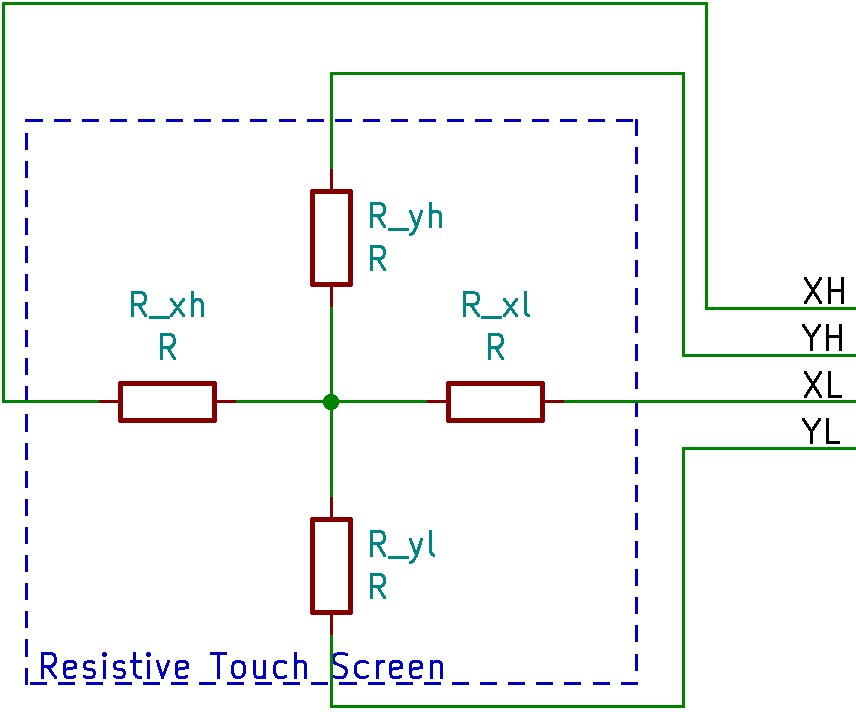
\includegraphics[width=0.6\linewidth]{fig/4-wire.jpg}
    \caption{Schemadarstellung eines 4-Wire resistiven Touchscreen}
    \label{fig:4w}
\end{figure}
\subsection{Arduino Leonardo Board}
Im Labor wurde hauptsächlich das Arduino Uno Board verwendet.
Die Unterschiede zwischen diesen beiden liegen darin, dass das Leonardo Board die Möglichkeit hat, sich als Peripherie an einem PC an zu melden.
Ermöglicht wird dies durch den Mikrocontroller ATmega32u4.
Der Mikrocontroller arbeitet nicht mit einem USB-Chip, sonder verarbeitet intern die serielle eingehende Daten und konvertiert diese für die Nutzung der USB-Schnittstelle.

